%!TEX program = pdflatex

\documentclass[12pt,a4paper]{report}
 
\usepackage[top=3cm, bottom=2cm, left=3cm, right=2cm,a4paper]{geometry}
\usepackage{setspace}
\usepackage{appendix}
\usepackage{verbatim}
%\singlespacing
\onehalfspacing 
%\doublespacing

\usepackage{indentfirst}

%\setlength{\parindent}{3.0cm}  % Altere o espaçamento do parágrafo aqui.

\usepackage[brazil]{babel}
\usepackage[utf8]{inputenc}
\usepackage{float}
\usepackage{graphicx,psfrag}
\newcommand\cincludegraphics[2][]{\raisebox{-0.3\height}{\includegraphics[#1]{#2}}}

\usepackage{multirow}

\usepackage{hyperref}
\hypersetup{
    colorlinks,
    citecolor=black,
    filecolor=black,
    linkcolor=black,
    urlcolor=black
}

\usepackage[T1]{fontenc}
%\usepackage{palatino}
\usepackage{amsmath, amsfonts, amssymb, amsthm}
\usepackage{xcolor}
\usepackage{url}
\usepackage{subcaption}
\usepackage{caption}
%\usepackage[all]{xy}
\usepackage[abnt-etal-list=0,abnt-etal-text=it,abnt-and-type=&,abnt-emphasize=bf,abnt-full-initials=yes,alf,bibjustif,abnt-repeated-author-omit=yes]{abntcite}

\usepackage{helvet}
\renewcommand{\familydefault}{\sfdefault}

\bibliographystyle{abntex2-alf}


\newtheorem{teorema}{Teorema}[chapter]
\newtheorem{lema}[teorema]{Lema}
\newtheorem{corolario}[teorema]{Corolário}
\newtheorem{proposicao}[teorema]{Proposi\c{c}\~ao}
\newtheorem{definicao}[teorema]{Defini\c{c}\~ao}
\theoremstyle{definition}
\newtheorem{exemplo}{Exemplo}
%\theoremstyle{remark}
\newtheorem*{obs}{Observação}

\newcommand{\R}{\mathbb{R}}
\newcommand{\Z}{\mathbb{Z}}
\newcommand{\F}{\mathbb{F}}
\newcommand{\I}{\mathbb{I}}
\newcommand{\LL}{\mathbb{L}}
\newcommand{\M}{\mathbb{M}}
\newcommand{\G}{\mathbb{G}}
\newcommand{\X}{\mathbf{X}}
\newcommand{\Y}{\mathbf{Y}}
\newcommand{\PX}{\mathcal{P}\left(\mathbf{X}\right)}
\newcommand{\FX}{\mathcal{F}\left(\X\right)}

\newcommand{\bb}{\begin{equation}}
\newcommand{\ee}{\end{equation}}
\newcommand{\bbb}{\begin{eqnarray}}
\newcommand{\eee}{\end{eqnarray}}
\newcommand{\benu}{\begin{enumerate}}
\newcommand{\eenu}{\end{enumerate}}
\newcommand{\tr}{\mbox{tr}}
\newcommand{\cao}{\c{c}\~ao }
\newcommand{\coes}{\c{c}\~oes }

\newcommand{\vetx}{\mathbf{x}}
\newcommand{\vety}{\mathbf{y}}
\newcommand{\vetw}{\mathbf{w}}
\newcommand{\vetn}{\mathbf{n}}
\newcommand{\ima}{\mathbf{a}}
\newcommand{\ims}{\mathbf{s}}
\newcommand{\imb}{\mathbf{b}}
\newcommand{\imt}{\mathbf{t}}

\newcommand{\alphav}{\mbox{\boldmath$\alpha$}}
\newcommand{\betav}{\mbox{\boldmath$\beta$}}
\newcommand{\thetav}{\mbox{\boldmath$\theta$}}
\newcommand{\lambdav}{\mbox{\boldmath$\lambda$}}
\newcommand{\gammav}{\mbox{\boldmath$\gamma$}}
\newcommand{\varthetav}{\mbox{\boldmath$\vartheta$}}
\newcommand{\nuv}{\mbox{\boldmath$\nu$}}
\newcommand{\sigmav}{\mbox{\boldmath$\sigma$}}

\newcommand{\tn}{\,\mathrm{t}\,}
\newcommand{\sn}{\,\mathrm{s}\,}
\newcommand{\agg}{\,\mathrm{a}\,}
\newcommand{\cc}{\, \mathtt{c} \,}
\newcommand{\bpm}{\begin{bmatrix}}
\newcommand{\epm}{\end{bmatrix}}

% \renewcommand{\rmdefault}{phv} % Arial
% \renewcommand{\sfdefault}{phv} % Arial

\usepackage[toctitles]{titlesec}
\titleformat{\chapter}
  {\normalfont\bfseries}{\thechapter}{1em}{\uppercase}
\titleformat{\section}
  {\normalfont\bfseries}{\thesection}{0.7em}{\sc}
\titleformat{\subsection}
  {\normalfont\bfseries}{\thesubsection}{0.4em}{ }


\newcommand{\capitulo}[1]{\chapter{\MakeUppercase{#1}}}
\newcommand{\secao}[1]{\section{\bf #1}}
\newcommand{\subsecao}[1]{\subsection{\bf #1}}

\titlespacing{\chapter}{0cm}{1cm}{1cm}

\usepackage{fancyhdr}
\pagestyle{fancy}
\lhead{}
\chead{}
\rhead{\thepage}
\lfoot{}
\cfoot{}
\rfoot{}
\renewcommand{\headrulewidth}{0pt}

\usepackage{tocloft}
\renewcommand{\cftpartleader}{\cftdotfill{\cftdotsep}} % for parts
\renewcommand{\cftchapleader}{\cftdotfill{\cftdotsep}} % for chapters
\renewcommand{\cftsecleader}{\cftdotfill{\cftdotsep}} % for sections

\makeatletter
\renewcommand\chapter{\if@openright\cleardoublepage\else\clearpage\fi
                    \thispagestyle{fancy}%
                    \global\@topnum\z@
                    \@afterindentfalse
                    \secdef\@chapter\@schapter}
\makeatother

\renewcommand{\chaptermark}[1]{%
\markboth{\thechapter.\ #1}{}}
\setlength{\headheight}{15pt}

\addto\captionsbrazil{\renewcommand{\contentsname}{}}
\addto\captionsbrazil{\renewcommand{\listfigurename}{}}
\addto\captionsbrazil{\renewcommand{\listtablename}{}}
\addto\captionsbrazil{\renewcommand{\bibname}{}} %inclui as configurações

% Escolhe a cor do tema do documento
\newcommand\CorTema{purple}
\newcommand\Revisao{1}

% Add if conditional, for put answers of the questions
\newif\ifanswers
\answerstrue % comment out to hide answers

\begin{document}

%
% CAPA
%
\thispagestyle{empty}

\begin{center}
    
\includegraphics[scale=0.7]{fig/logo.png}

    \vspace{.7cm}

    {\Large \uppercase{Pablo Jean Rozario}}

    \vspace{3cm}

    \Large \MakeUppercase{\textbf{PLANO DE AULA \\
            Microcontroladores - Turma 1 }}

    \vspace{3cm}

    \normalsize

    \begin{itemize}
        \item \textbf{Aula} : 1
        \item \textbf{Turma} : 1
        \item \textbf{Duração} : 4 Horas
        \item \textbf{Tema} : Apresentação e Conceitos
    \end{itemize}

    \vspace{3cm}

    Cambé - PR \\ Dezembro de 2021 \\ Revisão \Revisao
\end{center}

\newpage

% Blank Page

\thispagestyle{empty}
\mbox{}
\newpage

%
% Criação dos índices.
%

\begingroup
\let\clearpage\relax
\newpage
\begin{center}
    \MakeUppercase{\bf Sumário}
\end{center}
\tableofcontents
\thispagestyle{empty}

\newpage
\begin{center}
    \MakeUppercase{\bf Lista de Figuras}
\end{center}
\listoffigures
\thispagestyle{empty}


\newpage

\chapter{Objetivos}

\section{Objetivo Geral}

Apresentar aos estudantes os conceitos básicos do microcontrolador e o kit que será utilizado durante o Módulo.

\section{Objetivos Específicos}

\begin{itemize}
    \item Compreender a diferença entre as principais arquiteturas de microcontroladores e a aplicação em Sistemas Embarcados;
    \item conhecer alguns modelos de microcontroladores de diferentes fabricantes;
    \item apresentar o kit da STMicroeletronics \textit{NUCLEO-G0B1RE} que será trabalhado na disciplina.
\end{itemize}


\chapter{Metodologia}

\section{Introdução}

No inicio da disciplina, me apresentarei, de forma bem curta e rápida, e em sequência resumirei o que pretendemos trabalhar durante o curso. Sendo utilizado como base a tabela \ref{table:conteudo}.

\begin{table}[H]
    \centering
    \caption{Cronograma planejado para o curso de Microcontroladores.}
    \begin{tabular}{c|c|c|c}
    \textbf{Aula} & \textbf{Descrição}                                                                                                      & \textbf{Aula} & \multicolumn{1}{c}{\textbf{Descrição}}      \\ \hline \hline
    \textbf{1}       & \begin{tabular}[c]{@{}c@{}}Apresentação de Conceitos\\ Apresentação do kit STM32\end{tabular}                           & \textbf{7}       & Atividades                                   \\ \hline
    \textbf{2}       & \begin{tabular}[c]{@{}c@{}}Tipos especiais de (u)int\\ Registradores e Clock do uC\\ Entradas e Saídas IOs\end{tabular} & \textbf{8}       & Comunicação Serial I²C                       \\ \hline 
    \textbf{3}       & \begin{tabular}[c]{@{}c@{}}Estruturas em C\\Interrupções em IOs\end{tabular}                        & \textbf{9}       & Timers e RTC                                 \\ \hline
    \textbf{4}       & Conversor A/D e Interrupções                                                                                            & \textbf{10}      & PWM                                          \\ \hline
    \textbf{5}       & Comunicação Serial UART                                                                                                 & \textbf{11}      & \multirow{2}{*}{Desenvolvimento de Projetos} \\ \cline{1-3}
    \textbf{6}       & Comunicação Serial SPI                                                                                                  & \textbf{12}      &                                              \\
    \end{tabular}
\label{table:conteudo}
\end{table}

Apresentarei algumas questões questões aos alunos, tais como, "O que é o microcontrolador?" e "Qual a importância dos microcontroladores em nossas vidas". Após as resposta da turma, será respondido que, respectivamente:

"O microcontrolador é um componente eletrônico composto de um processador e periféricos em um único encapsulamento, capaz de executar um programa previamente gravado".

"A importância dos microcontroladores em nossas vidas está na automatização de diversos equipamentos que utilizamos e ainda de dispositivos que carregamos no dia a dia que são dotados de certa autonomia e inteligência, tais como \textit{smartwatch's} e \textit{smartphones}."

\begin{figure}[H]
    \centering
    \caption{Exemplos de aplicação de sistemas embarcados.}
    \begin{subfigure}{.4\textwidth}
      \centering
      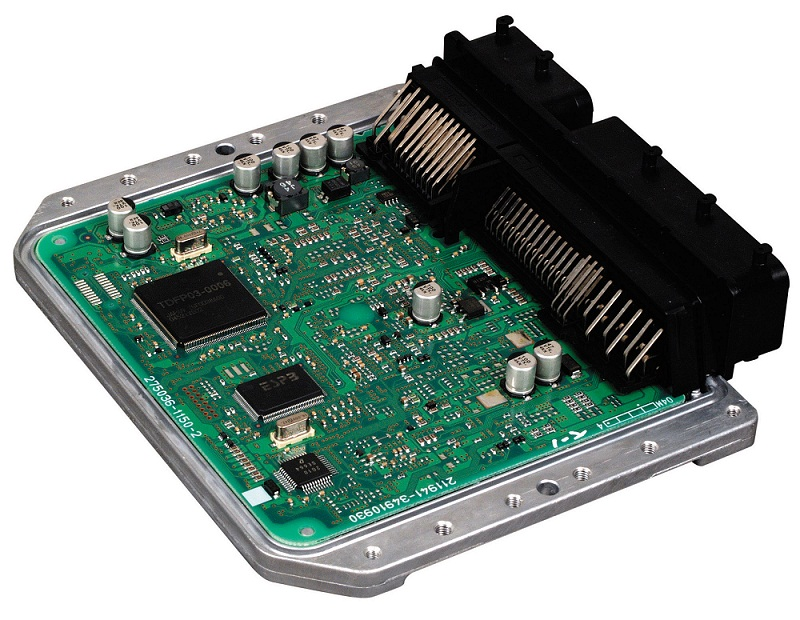
\includegraphics[width=1\linewidth]{fig/ECU.png}
      \caption{Central Eletrônica (ECU) de um carro.}
      \label{fig:example_ECU}
    \end{subfigure}%
    \begin{subfigure}{.4\textwidth}
      \centering
      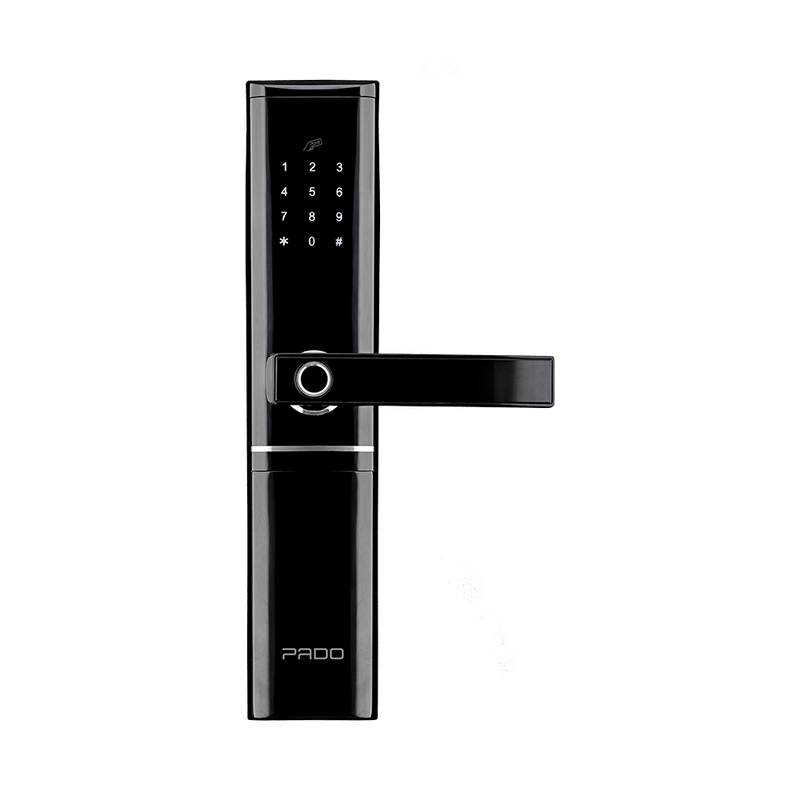
\includegraphics[width=1\linewidth]{fig/fd500.png}
      \caption{Fechadura eletrônica.}
      \label{fig:example_missle}
    \end{subfigure}
    \begin{subfigure}{.4\textwidth}
      \centering
      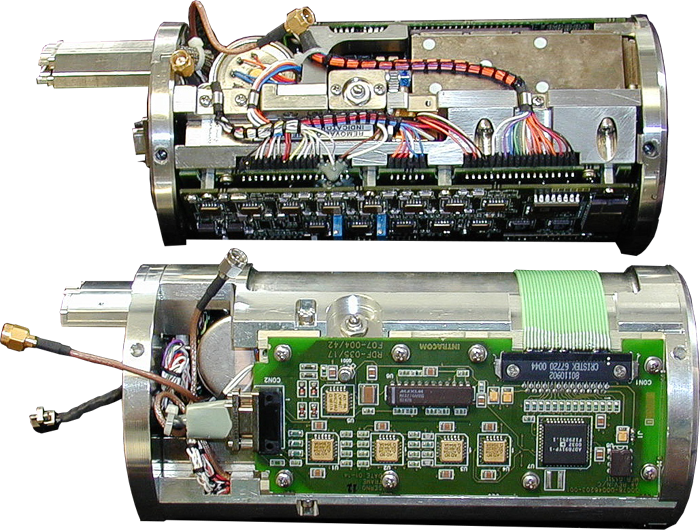
\includegraphics[width=1\linewidth]{fig/missile_module.png}
      \caption{Módulo de Controle de um Míssil.}
      \label{fig:plot_p8d25i0_025}
    \end{subfigure}
    \begin{subfigure}{.4\textwidth}
      \centering
      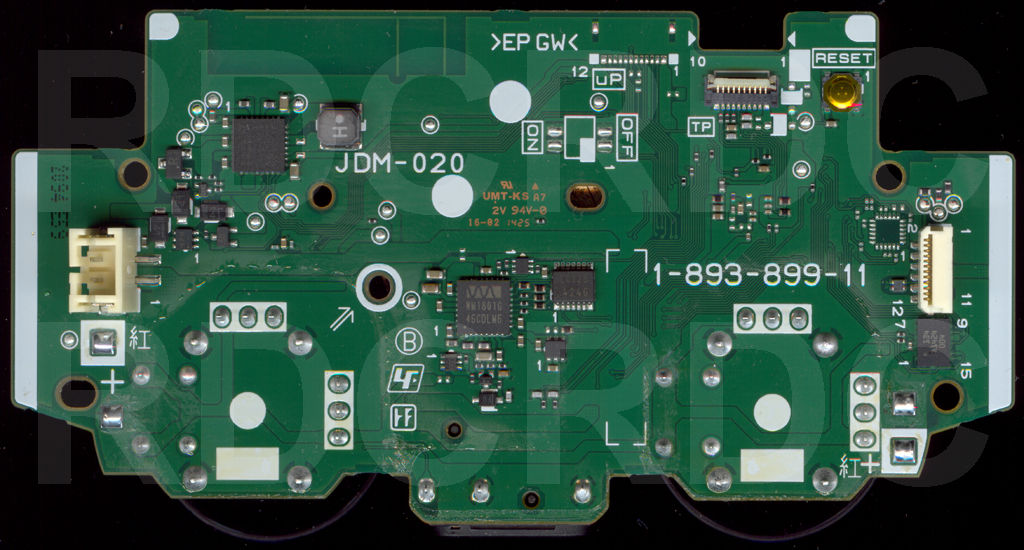
\includegraphics[width=1\linewidth]{fig/ps4_controller.png}
      \caption{Placa eletrônica de um controle de PS4.}
      \label{fig:plot_p8d35i0_05}
    \end{subfigure}
    \caption*{Fonte: Google imagens.}
    \label{figura:application_examples}
    \end{figure}

Com estas resposta, será apresentado exemplos de produtos e aplicações dos microcontroladores, desde eletrodomésticos e brinquedos, até sistemas bélicos. Pois é importante que o estudante tenha noções de onde pode ser aplicado estes dispositivos.

Será apresentado também a figura , com finalidade de exemplificar como é a estrutura interna de um microcontrolador.

\begin{figure}[H]      % Aqui inicia o ambiente de figura
\begin{center}		   % centraliza a figura
\caption{Diagrama de blocos de um microcontrolador.}		% insere a legenda da figura
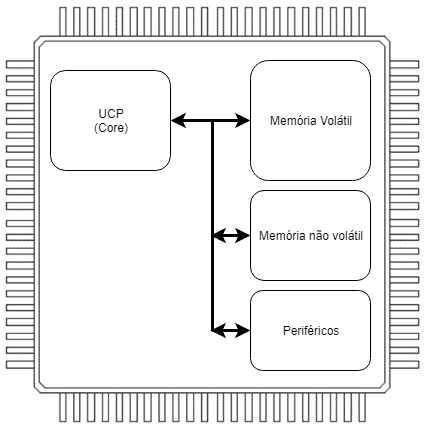
\includegraphics[scale=0.5]{fig/basic_microcontroller.png}
\caption*{Fonte: Google imagens.}
\label{fig:basic_microcontroller}
\end{center}
\end{figure}

Na figura \ref{fig:architecture_microcontroller} tem-se por objetivo exibir de forma um pouco mais detalhada a estrutura de um microcontrolador, buscando fornecer aos estudantes uma compreensão de como os dados fluem internamente.

\begin{figure}[H]      % Aqui inicia o ambiente de figura
    \begin{center}		   % centraliza a figura
    \caption{Diagrama do barramento de um microcontrolador.}		% insere a legenda da figura
    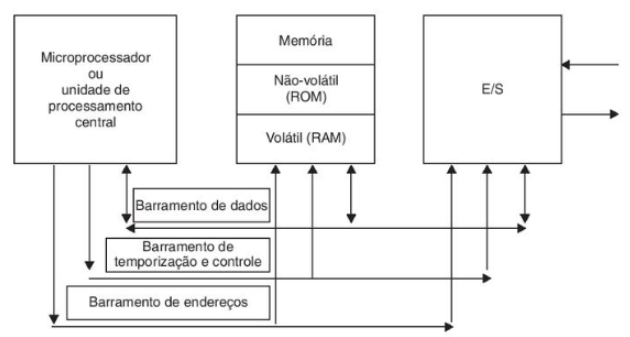
\includegraphics[scale=0.5]{fig/architecture_microcontroller.png}
    \caption*{Fonte: \cite{ci:microcontroller_8051}.}
    \label{fig:architecture_microcontroller}
    \end{center}
\end{figure}

Deverá ser explicado que o \textbf{Barramento de temporização e controle} é responsável por definir o endereço do dispositivo de IO no barramento de endereços por um período de tempo definido, além do sentido (leitura ou escrita). O \textbf{Barramento de endereços} tem por objetivo informar ao periférico o endereço da informação que deseja alterar ou ler. E por fim, o \textbf{Barramento de dados} é por onde é disponibilizada a informação.

\textbf{Dica Didática} : Utilizar como exemplo, uma conversa com os alunos, onde falo com um e específicos pelo seu nome, e solicito,por exemplo, quantas bolinhas tem na caixa X, e da mesma forma, para outro aluno, digo para guardar Y bolinhas na caixa Z, como forma de ilustrar o barramento.

\section{Microcontrolador ou Microprocessador}

Durante a aula, será apresentada uma tabela \ref{table:microprocessorXmicrocontroller1} para apresentar os grandes pontos de diferença entre microcontroladores e microprocessadores.

\begin{table}[H]
    \centering
    \caption{Escolha entre microcontrolador e microprocessador.}
    \begin{tabular}{c|c|c}
    \textbf{Característica} & \textbf{Microprocessadores}                                                   & \textbf{Microcontrolador}                                                            \\ \hline
    \textbf{Periféricos}    & \begin{tabular}[c]{@{}c@{}}Necessita de periféricos\\ externos\end{tabular}   & \begin{tabular}[c]{@{}c@{}}Periféricos integrados\\ no chip\end{tabular}             \\ 
    \textbf{Memória}        & \begin{tabular}[c]{@{}c@{}}Permite vários formatos\\ de dados\end{tabular}    & \begin{tabular}[c]{@{}c@{}}Poucos tipos de dados (8, 16 ou\\ 32 bits)\end{tabular}   \\
    \textbf{Processamento}  & \begin{tabular}[c]{@{}c@{}}ALU Complexa e possui\\ coprocessador\end{tabular} & \begin{tabular}[c]{@{}c@{}}ALU limitada e ausência de\\ coprocessamento\end{tabular} \\ 
    \textbf{Custo}          & Custo elevado                                                                 & Baixo custo, a depender da plataforma                                                \\ 
    \textbf{Consumo}        & Alto consumo de enegeria                                                      & \begin{tabular}[c]{@{}c@{}}Possui métodos para economia de\\ energia\end{tabular}    \\ 
    \end{tabular}
\label{table:microprocessorXmicrocontroller1}
\end{table}

É importante ressaltar a importância de ter os parâmetros do projetos, não apenas para decidir entre Microcontrolador ou Microprocessador, mas também para definir a escolha do modelo do microcontrolador. 

Como existem vários fabricantes de microcontroladores e ainda, várias linhas dentro dos fabricantes, é importante saber definir qual microcontrolador será escolhido. Como forma de ilustrar isto, a tabela \ref{table:microcontrollers} irá indicar 4 exemplos de microcontroladores de diferentes capacidades.

\begin{table}[H]
    \centering
    \caption{Comparativo entre microcontroladores de várias linhas.}
    \begin{tabular}{c|c|c|c|c}
    \textbf{}           & \textbf{PIC16F1824} & \textbf{MSP430FR2433} & \textbf{STM32G0B1RE} & \textbf{CC2642R} \\ \hline
    \textbf{Fabricante} & Microchip           & Texas                 & ST                   & Texas            \\
    \textbf{Core}       & PIC16               & MSP430                & ARM M0+              & ARM M4F          \\
    \textbf{Bits}       & 8bits               & 16bits                & 32bits               & 32bits           \\
    \textbf{Flash}      & 7KB                 & 15.5K                 & 512KB                & 352KB            \\
    \textbf{RAM}        & 256B                & 4K                    & 144KB                & 80KB             \\
    \textbf{I/Os}       & 12                  & 19                    & 60                   & 31               \\
    \textbf{ADC}        & 10bits              & 10bits                & 12bits               & 12bits           \\
    \textbf{SPI}        & X                   & X                     & X                    & X                \\
    \textbf{I2C}        & X                   & X                     & X                    & X                \\
    \textbf{UART}       & X                   & X                     & X                    & X                \\
    \textbf{EEPROM}     & X                   & -                     & -                    & -                \\
    \textbf{Extra}      & -                   & FRAM                  & USB OTG              & Bluetooth        \\
    \end{tabular}
\label{table:microcontrollers}
\end{table}

Será importante apontar as diferenças entre as interfaces, principalmente com respeito as capacidades de memórias, que é um dos parâmetros que mais saltam aos olhos. E além destes pontos que estão na tabela, esclarecer que existem mais parâmetros, como quantidade e capacidade dos periféricos, clock máximo, recursos especiais e consumo energético.


\section{8bits ou 32bits}

Irei explicar o caso de como quase sempre se desenvolve em C, as diferenças ficam muito transparentes, pois o C irá abstrair muitas etapas das instruções dos microcontroladores, mas quando se trabalha com assembly, fica evidente alguns aspectos, como por exemplo, somar números de 32bits, em nível de assembly é bem simples em um microcontrolador de 32 bits, mas árduo em 8bits.

Informar também aos estudantes, que as diferenças estão mais no tamanho dos registradores, e do barramento, que será do tamanho da arquitetura do microcontrolador. Mas é importante ressaltar que, em tese um microcontrolador de 8 bits poderia endereçar até no máximo 256 bytes de ram/flash, no entanto, alguns microcontroladores possuem uma estratégia de paginação, permitindo ter um barramentos de 16bits para a flash, permitindo endereçar até 64KB.

\section{Arquitetura de Microcontroladores}

É importante desde o começo os estudantes ja terem em mente que existem duas arquiteturas de microcontroladores, para tal, será explicado de forma mais básica sobre cada uma das duas.

Em \cite{ci:von_neu_harv_diff} é explanado um pouco sobre cada uma das arquiteturas, podendo sugerir aos alunos, acesso a esta referencia, para buscar esta e mais informações.

\subsection{Von Neumann}

A arquitetura Von Neumann foi desenvolvida pelo Matemático e Físico John Von Neumann em 1945, é uma arquitetura que tem como base o conceito de armazenar os dados e as instruções em uma mesma memória. ou seja, a memória RAM e a Flash estão no mesmo barramento.

\subsection{Harvard}

Diferente da Von Neumann, na arquitetura Harvard, o barramento da memória de dados e da memória de programa é separada, ou seja, a RAM é separada da Flash.

Foi desenvolvida para superar o gargalo causado pela arquitetura Von Neumann na época.

Aprestarei a figura \ref{fig:compare_h_vn} onde é exibido o esquemático básico de uma arquitetura Von Neumann e uma Harvard.


\begin{figure}[H]      % Aqui inicia o ambiente de figura
\begin{center}		   % centraliza a figura
\caption{Esquemático de uma arquitetura Von Neumann e Harvard, respectivamente.}		% insere a legenda da figura
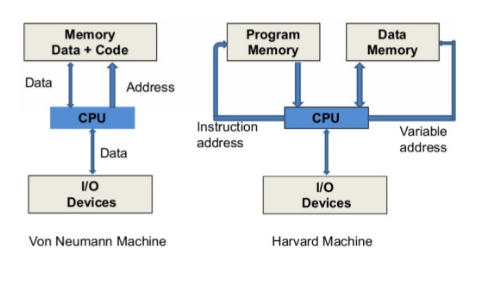
\includegraphics[scale=0.9]{fig/VN_Hardvard_compare.png}
\caption*{Fonte: Google Imagens.}
\label{fig:compare_h_vn}
\end{center}
\end{figure}

Pela figura, fica bem evidenciado a diferença das arquiteturas, onde o barramento de dados é compartilhado no Von Neumann, e separado na Harvard.

\subsection{Diferenças}

Não existe uma arquitetura melhor que a outra, ambas possuem vantagens e desvantagens, a depender da aplicação em que são empregados os microcontroladores. Em resumo, as diferenças são exibidas na tabela \ref{table:compare_vn_h}, que foi adaptada de \cite{ci:von_neu_harv_diff}.

\begin{table}[H]
\centering
\caption{Comparativo entre microcontroladores de várias linhas.}
    \begin{tabular}{|c|c|}
    \hline
    \textbf{Von Neumann}                                                                                                          & \textbf{Harvard}                                                                                          \\ \hline
    \begin{tabular}[c]{@{}c@{}}O mesmo endereço físico é\\  utilizado para memória de \\ programa e memória de dados\end{tabular} & \begin{tabular}[c]{@{}c@{}}Diferentes endereços físicos são\\ utilizados pelas memórias\end{tabular}      \\ \hline
    \begin{tabular}[c]{@{}c@{}}O barramento da memória de \\ programa e da memória de\\ dados é compartilhado\end{tabular}        & \begin{tabular}[c]{@{}c@{}}O barramentos das memórias\\ é isolado\end{tabular}                            \\ \hline
    \begin{tabular}[c]{@{}c@{}}É necessário pelo menos dois\\ ciclos de clock para executar\\ uma única instrução\end{tabular}    & \begin{tabular}[c]{@{}c@{}}Uma instrução pode ser\\ executada em um ciclo de\\ clock\end{tabular}         \\ \hline
    Possui custo menor                                                                                                            & \begin{tabular}[c]{@{}c@{}}Possui um custo mais elevado\\ se comparado a Von Neumann\end{tabular}         \\ \hline
    \begin{tabular}[c]{@{}c@{}}Não é possível acessar uma\\ instrução e ler/escrever ao\\ mesmo tempo\end{tabular}                & \begin{tabular}[c]{@{}c@{}}E possível ler/escrever ao mesmo\\ tempo que acessa uma instrução\end{tabular} \\ \hline
    \begin{tabular}[c]{@{}c@{}}Muito utilizado em computadores\\ e microcontroladores ARM\end{tabular}                            & \begin{tabular}[c]{@{}c@{}}Utilizado em microcontroladores\\ e processamento de sinais\end{tabular}       \\ \hline
    \end{tabular}
\label{table:compare_vn_h}
\end{table}

\section{Registradores}

Segundo \cite{ci:beginner_guide} registradores nada mais são do que locais de memória em que é possível realizar as operação de Escrita e/ou Leitura, como por exemplo a memória RAM, que nada mais é do vários registradores que podem ser lidos e escritos, que tem como característica serem velozes e perderem seus dados ao serem desenergizados.

Mas os microcontroladores possuem os SFRs, ou \textit{Special Function register}, que são, de forma similar a RAM, locais de memória que podem controlar diretamente o hardware do componente, ou o próprio hardware do microcontrolador pode controlalos, para indicar status.

Cada bit do SFR é designado a uma função, este podendo ser um \textit{Control bit} ou um \textit{Flag bit}. Os \textit{Control bits} são como se fossem chaves que acionam determinadas funções do hardware, ou configuram, alguns necessitando apenas de um bit, como um \textbf{enable} para uma interface serial, ou vários bits, como definir um \textit{prescaler}. Um \textit{Flag bit} é controlado diretamente pelo hardware, e seu objetivo é indicar alguma status ou evento que ocorreu no microcontrolador, como, por exemplo, indicar que uma interrupção em um pino de entrada.

Na figura \ref{fig:srf_example} será exibido aos estudantes um diagrama para exemplificar três SFRs de um determinado microcontrolador.

\begin{figure}[H]      % Aqui inicia o ambiente de figura
    \begin{center}		   % centraliza a figura
    \caption{Esquema de três SFRs.}		% insere a legenda da figura
    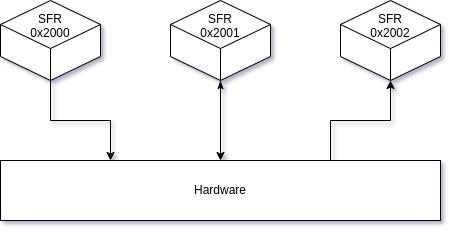
\includegraphics[scale=0.65]{fig/sfr_example.png}
    \caption*{Fonte: Autoria própria.}
    \label{fig:srf_example}
    \end{center}
\end{figure}

Todas as informações dos SFRs estão nos datasheets dos componentes, explicitando cada bit de cada registrador, se podem ser lidos e/ou escritos.

Na figura \ref{fig:gpio_port_mode} tem-se um exemplo de registrador que configura o modo de operação de uma GPIO de um microcontrolador, neste exemplo estamos tomando o registrador do STM32G0B1RE, que está disponível em \cite{ci:rm0444}.


\begin{figure}[H]      % Aqui inicia o ambiente de figura
    \begin{center}		   % centraliza a figura
    \caption{Esquemático de uma arquitetura Von Neumann e Harvard, respectivamente.}		% insere a legenda da figura
    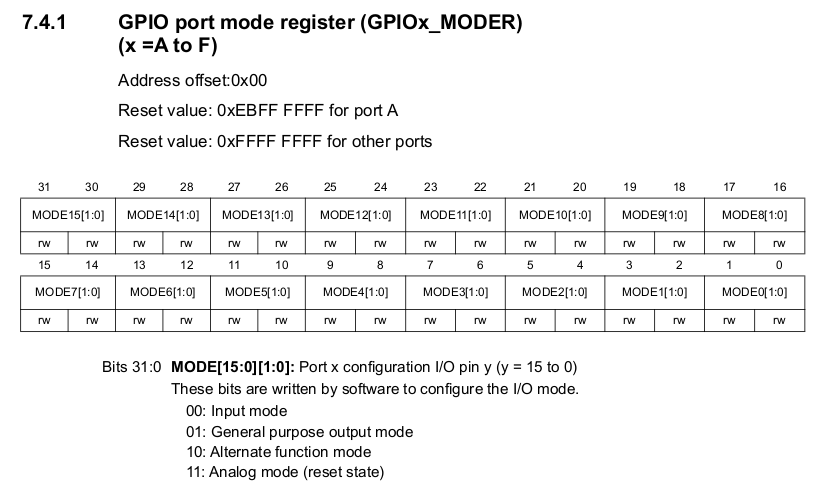
\includegraphics[scale=0.5]{fig/gpio_port_mode.png}
    \caption*{Fonte: \cite{ci:rm0444}}
    \label{fig:gpio_port_mode}
    \end{center}
\end{figure}

Nesta figura, será relevante apontar que o documento especifica cada bit do registrador, se suporta leitura e/ou escrita, descrição dos elementos do registrador e o valor do reset do registrador.

\subsection{Program Counter e a Stack}

Ainda tomando como base \cite{ci:beginner_guide}, é importante citar que o contador de programa (\textit{Program Conter} ou simplesmente PC) é um ponteiro que diz para a CPU onde se encontra a próxima instrução a ser executada.

No momento do POR (\textit{Power On Reset}) o contador de programa inicia no endereço $0x0000$, e é incrementado automaticamente ao carregar a instrução, sendo então $0x0001$.

O PC é incrementado automaticamente em 1 a cada instrução executada, até o momento em que o mesmo é modificado pelo programa (causando um \textit{jump}) ou em chamadas de funções, que também realizam um salto no programa, mas que faz uso da \textit{Stack}.

Neste ponto, é interessante apresentar o problema antes de falar da \textit{stack}, após apresentar e questionar sobre, partir para explanação.

A \textit{stack} é uma pilha que é utilizada pelas chamadas de subrotinas, realizando o armazenamento do próximo endereço da chamada da subrotina. A mesma função na lógica de LIFO (\textit{Last In, First Out}) para armazenar os valores para retorno.

Durante a operação, ocorre os seguintes passos:

\begin{enumerate}
    \item É feito o PUSH na stack do valor do PC na chamada de subrotina ou interrupção;
    \item o PC é modificado com o endereço de onde inicia a execução da subrotina ou interrupção;
    \item o programa então pula e executa a subrotina;
    \item quando ocorre a chamada de \textit{return}, é realizado o POP na pilha e o valor atribuído ao PC;
    \item o PC retorna a próxima instrução antes da chamada da função ou da ocorrência da interrupção.
\end{enumerate}

Na figura \ref{fig:stack_pointer} é exemplificado o funcionamento de uma Stack.

\begin{figure}[H]      % Aqui inicia o ambiente de figura
    \begin{center}		   % centraliza a figura
    \caption{Exemplo de operação de uma stack.}		% insere a legenda da figura
    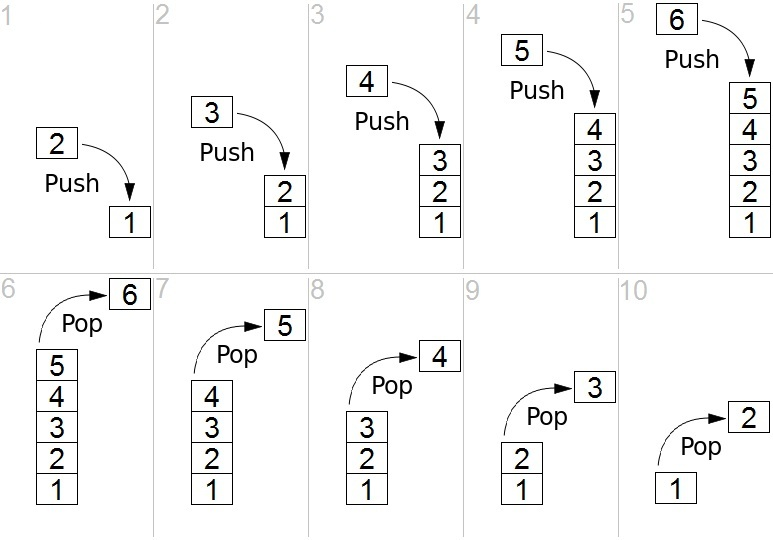
\includegraphics[scale=0.6]{fig/stack_pointer.jpg}
    \caption*{Fonte: Google imagens.}
    \label{fig:stack_pointer}
    \end{center}
\end{figure}

Um microcontrolador pode implementar a stack de duas formas: Por software e por Hardware. Por software, como é o caso de linhas como STM8, STM32 e entre outras, a stack é armazenada na memória RAM e pode ser definida pelo desenvolvedor no programa, tem por vantagem ser be flexível, mas parte da memória RAM é perdida.

Já por hardware, a stack é implementada através de registradores dedicados à esta funcionalidade, como é o caso da linha PIC da Microchip, a grande vantagem é que não é necessário reservar memória RAM para a funcionalidade, mas o tamanho da \textit{stack} é limitado ao que o hardware oferece.

\section{Set de Instruções}

É importante falar aos estudantes que o conjunto de instruções ou \textit{instruction set} engloba todas as instruções que são compreendidas pelo microcontrolador, que nada mais são do que as operações que o microcontrolador pode fazer e que possui implementado em seu hardware.

Quando um programa é compilado e gravado no microcontrolador, o binário gerado nada mais é do que a sequência de instruções geradas para atingir a finalidade desejada. Abaixo tem-se um exemplo de instruções para o \textit{core} PIC18.

\begin{verbatim}
    MOVLW 10H        ; Set 0x10 to the WREG
    MOVF  20H, 1, 0  ; Move 0x10 to the address 0x20   
    MOVLW 5H         ; Set 0x5 to the WREG
    ADDWF 20H, 1, 0  ; Sum WREG with value on 0x20 
                     ; (0x10+0x5) and stores in 0x20
\end{verbatim}

Cada microcontrolador possui seu \textit{set} de instruções específicos da \textit{CPU}, estes sets são divididos em dois principais grupos, \textbf{RISC} (\textit{Reduced Instruction Set Computer}) e \textbf{CISC} (\textit{Complex Instruction Set}).

\begin{itemize}
    \item \textbf{RISC} : Arquitetura com pequeno conjunto de instruções mais simples, sendo mais baratos de produzir e permitem um \textit{clock} mais alto pela simplicidade dos circuitos internos. Geralmente é associado a arquitetura Harvard.
    \item \textbf{CISC} : Arquitetura com uma grande gama de instruções, sendo algumas instruções feita por "microprogramas" gravados na cpu, possuindo ainda unidades de controle poderosas. Geralmente é associado a arquitetura Von Neumann.
\end{itemize}

Como exemplos, temos a linha PIC e ARM com arquiteturas RISC, e em contraponto, temos a linha 8051 que é baseada em arquitetura RISC. É interessante informar aos estudantes que em \cite{ci:cortex_m0_iss} é possível ter acesso as instruções do núcleo.

\section{Kit de Desenvolvimento NUCLEO-G0B1RE}

Após apresentar um básico sobre microcontroladores, apresentar o kit que iremos utilizar para as aulas o kit da ST Microeletronics, a \textbf{NUCLEO-G0B1RE}, que possui um STM32G0B1RE com um debugger já na placa. Possuindo também terminais de I/Os para ligar com circuitos externos, como botões, LEDs, circuitos integrados e etc.

na figura \ref{fig:nucleog0b1re} temos a foto de um exemplar do kit de desenvolvimento.

\begin{figure}[H]
    \begin{center}
    \caption{NUCLEO-G0B1RE, kit de desenvolvimento da ST Microeletronics.}		% insere a legenda da figura
    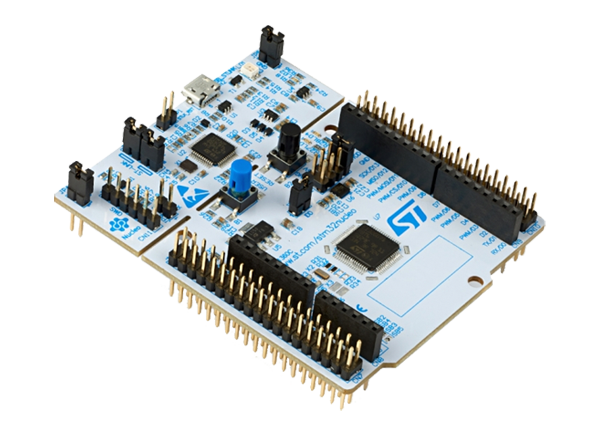
\includegraphics[scale=0.6]{fig/nucleog0b1re.png}
    \caption*{Fonte: Google imagens.}
    \label{fig:nucleog0b1re}
    \end{center}
\end{figure}

Possui como principais características, além das citadas na tabela \ref{table:microcontrollers}:

\begin{itemize}
    \item Unidade de cálculo de CRC;
    \item RTC alimentado por bateria;
    \item controlador DMA;
    \item DACs de 12bits;
    \item 15 timers;
    \item três interfaces I2C;
    \item seis interfaces USART;
    \item três UART de baixo consumo;
    \item três SPI;
    \item HDMI interface;
    \item USB OTG.
\end{itemize}

Outras informações podem ser acessadas em \cite{ci:um2324}, e neste momento distribuir uma versão impressora do documento para cada estudante, para que sempre tenham em mãos informações do \textit{hardware} da placa. 

\section{Sistema de Clocks}

Será abordado sobre o sistema de clocks do microcontrolador, sendo apresentado através do arquivo CubeMX (.ioc) na própria IDE, descrevendo apenas os blocos mais relevantes.

Aqui, destacar que o \textbf{ciclo de máquina} corresponde a um múltiplo do dos ciclos de clock, o que representa quantos ciclos são necessários para executar uma instrução. Por exemplo, microcontroladores PIC requerer 4 ciclos de clock para executar uma instrução.

\section{IDE de Desenvolvimento - STM32CubeIDE}

Será realizada a instalação da ferramenta \textbf{STM32CubeIDE}, que será utilizada para desenvolver as atividades no kit. 

A instalação será feita na distro Ubuntu, do Linux, que é o Sistema Operacional que está instalado nas máquinas.

Se possível, será rodado um firmware exemplo apenas para verificar se o software e as ferramentas de debugger estão funcionando adequadamente e para apresentar como é realizado o debug.

\begin{figure}[H]
    \begin{center}
    \caption{Logo do STM32CubeIDE.}		% insere a legenda da figura
    
\includegraphics[scale=0.6]{fig/stm32cubeide.png}
    \caption*{Fonte: Google imagens.}
    \label{fig:stm32cubeide}
    \end{center}
\end{figure}


\chapter{Recursos Didáticos}

Será utilizado lousa e canetas apropriadas, computador com os softwares necessários e projetor.

\chapter{Forma de Avaliação}

Avaliação será feita através das listas de exercícios para serem resolvidas durante as aulas ou no horário reservado.

\newpage

\chapter{Histórico de Revisão}

\subsection*{Revisão 1}

Primeiro documento.

\newpage

\begin{appendices}

    \chapter{Anexos}

    \section{Lista de Exercícios - Resolvida}
    % Macros auxiliares

\newcounter{idx}
\setcounter{idx}{1}

\newcommand{\question}[1]{ 

    \textbf{\theidx : }#1
    \stepcounter{idx}
}

\newcommand{\answer}[1]{

    \ifanswers
    {
        %\newline
        \scriptsize\color{purple}\textbf{R:} #1
    }
    \else
    \vspace{1cm}
    \fi 
}

% Cabeçalho para a Lista de Exercícios
\begin{tabular}{l|ll}
    \multirow{3}{*}{
\includegraphics[width=84px]{fig/logo.png}} & { } & {\LARGE \textbf{Lista de Exercícios \#1 }} \\
    & { } & {\Large Pado Labs - Microcontroladores} \\
    & { } & {Introdução aos microcontroladores}   
    \end{tabular}
    
    \vspace{0.5cm}
    \textit{Tips and Tricks} : Utilizar o \textit{User Manual UM2324} para resolver as questões.

    \textit{Requirements} : Resolva todos os exercícios.
    \vspace{0.5cm}

    \question{Além dos exemplos citados em sala, poderia citar mais exemplos de aplicação de microcontroladores?}

    \answer{Mouse, teclado, microondas, televisão, roteador, etc.}


    \question{Qual a principal diferença entre as memórias voláteis e memórias não voláteis?}

    \answer{A memória volátil perde os dados armazenados ao ser desligada, enquanto que as não voláteis retém os dados mesmo após ser desenergizado.}


    \question{Explique a diferença do barramento de endereço para o barramento de controle de um microcontrolador.}

    \answer{O barramento de endereços indica qual a posição da informação a ser alterada ou requerida do periférico, enquanto que o barramento de controle seleciona o periférico desejado e se a operação é leitura ou escrita.}

    
    \question{Você é um projetista de uma empresa que está desenvolvendo um novo produto que necessitará de um dispostivo programável para efetuar um controle. Este produto tem como alicerce o baixo custo e processamento relativamente pequeno. Tomando isto, é possível que o microcontrolador que melhor se encaixar na sua aplicação seja um de arquitetura \textit{Von Neumann} ou \textit{Harvard}?}

    \answer{Von Neumann, pois são mais baratos de serem produzidos.}


    \question{Aproveitando a questão anterior, fale sobre a arquitetura Harvard.}

    \answer{A Arquitetura Harvard tem por grande diferença, ter a memória de dados e a memória de programas separadas, o que implica em melho performance das instruções, mas em um custo mais elevado, além de impossibilitar executar instruções da memória RAM.}


    \question{É verdade que o tamanho do barramento de dados (bits) de um microcontrolador é suficiente para escolher um modelo para aplicar em um projeto? Justifique.}

    \answer{Não, pois é necessário também observar outros parâmetros como quantidade de memórias, periféricos e entre outros parâmetros.}


    \question{Explique o que são os SRFs.}

    \answer{SFRs são os registrados de funções especiais, que estão conectados ao hardware do microcontrolador, e tem por função controlar funcionalidades do microcontrolador (\textit{control bit} ou indicar algum status (\textit{flag bit})).}


    \question{O que ocorre com o microcontrolador caso a \textit{stack} estoure?}

    \answer{O microcontrolador, em geral, força um reset quando ocorre o estouro da \textit{stack}.}


    \question{O contador de programa pode ser alterado durante a execução dos programas, cite em que pontos que podem ocorrer a alteração do contador de programa.}

    \answer{O PC pode ser alterado na ocorrência de uma interrupção, na chamada de uma subrotina ou ao chamar a função de \textit{return}, que realiza o \textit{pop} da stack.}


    \question{Qual a ordem de entradas e saídas da stack?}

    \answer{Pelo sistema de LIFO, \textit{Last In First Out}, ou seja, quem entrou por último, sai primeiro.}

    \question{Tomando como base a questão anterior, esboce o funcionamento de uma stack.}

    \answer{Diagrama similar ao apresentado nos slides.}


    \question{Qual a grande vantagem de se utilizar uma \textit{stack} po software?}

    \answer{É mais flexível, pois permite que o tamanho seja configurado de acordo com a necessidade.}

    \question{A arquitetura RISC permite o microcontrolador operar com \textit{clocks} mais elevados, qual o motivo deste fato?}

    \answer{Como os circuitos internos de uma arquitetura RISC são mais simples, é possível atingir maiores velocidades de processamento.}

    
    \question{Quais conhecimentos você possuia previamente sobre o tema microcontroladores?}

    \answer{Pessoal.}
    

    \question{Já trabalhou com microcontroladores? Conte quais e o qual sua opinião sobre eles?}

    \answer{Pessoal.}
    

    \question{O kit contém LEDs que podem ser controlados pelo programa, quantos este kit nos disponibiliza}

    \answer{O kit disponibiliza um LED para ser controlado pelo programa, indicado pela legenda LD4.}
    

    \question{Vemos que o kit possui dois botões, um azul e um preto, qual o uso de cada um deles?}

    \answer{O botão USER é ligado em uma entrada do microcontrolador, e sua função é definida pelo desenvolvedor, enquanto que o RESET é ligado ao pino de reset do microcontrolador.}
    

    \question{A memória flash é onde o microcontrolador armazena os comandos a serem executados, parâmetros de configuração e ainda pode ser utilizada para armazenar dados (memória não volatil). Quantos de capacidade nosso microcontrolador possui?}

    \answer{Na página 8 do documento UM2324, podemos ver que o microcontrolador possui 512KB de memória flash.}
    

    \question{Ao observar a placa, vemos que a mesma possui dois microcontroladores, um sendo o STM32G0B1RE e o outro se trata de um STM32F103CB. Qual a função do ultimo microcontrolador?}

    \answer{O STM32F103 é o microcontrolador que tem implementar o ST-Link V2, se tratando do debugger que é utilizado para gravar o microcontrolador e realizar o debug.}
    

    \question{O kit possui um debugger integrado, que possui um interface serial auxiliar e a interface de gravação e debug do microcontrolador, qual o nome desta interface e quais o terminais dessa interface?}

    \answer{A interface e chamada de SWD (Serial Wire Debug), os terminais do SWD são o SWCLK (clock) e SWDIO (entrada e saída de dados), além do RESET e dos pinos de alimentação do conector CN11.}
    

    \question{Este kit permite que utilizemos  debugger para gravar um microcontrolador externamente (em outra placa, por exemplo), no entanto o que é necessário ser feito e qual conector que é utilizado para realizar esta função?}

    \answer{Remover os Jumpers do CN4 e remover o SB19, que fica no bottom layer da placa.}
    

    \question{O kit vem de fábrica com um programa exemplo. Descreva o que este programa teste faz.}

    \answer{O programa exemplo pisca o LED LD4 em uma frequência constante, que é alterada ao pressionar o botão USER.}
    

    \question{É possível alimentar o kit com 4 formas de alimentação, cite-as e indique como liga-lás de forma adequada.}

    \answer{5V\_USB\_STLK, alimentação oriunda do conector USB, o jumper JP2 deve estar nos pinos 1 e 2. VIN, alimentação que suporte de 7 à 12V, o jumper deve estar no pino 3 e 4 do JP2, e a alimentação deve entrar no pino 24 do CN7 ou pino 8 do CN6. O E5V é a alimentação de 5V que pode vir externamente, o Jumper deve estar no pino 5 e 6 do JP2 e alimentar pelo pino 6 do CN7. 5V\_USB\_CHARGER, alimentação oriunda do USB, assim como o 5V\_USB\_STLK, a diferença é que o debugger é desabilitado e, como não há o controle de corrente, o USB do dispositivo que esta provendo a alimentação pode ser danificado, para habilitar o JP2 deve estar com o Jumper na posição 7 e 8.}

    
    \question{Cite as fontes de clock que o kit permite utilizar e seus respectivos usos.}
    
    \answer{LSE, cristal de 32.758kHz utilizado pelo RTC. MCO, sinal de 8MHz gerado pelo ST-Link. HSE, cristal de 8MHz, não implementado no kit, sendo necessário adquiri-lo e solda-lo manualmente.}
    

    \question{Cite as fontes de reset que o kit permite utilizar para resetar o microcontrolador.}
    
    \answer{Botão B2 (RESET), através do ST-Link, pelo pino 3 do CN6 e através do pino 14 do CN7.}
    

    \question{O ST-Link do kit implementa uma porta COM virtual (serial) através do USB, está porta virtual consome qual periférico do STM32? O Manual UM2324 ainda informa que é possível isolar o periférico, qual é o procedimento?}
    
    \answer{Utiliza o periférico UART2. Para isolar a UART2 da porta COM é necessário desabilitar o SB16 e SB18.}
    

    \question{O kit possui 4 LEDs, denote a função de cada um dos LEDs.}
    
    \answer{O LED LD1 é um led bi-color que indica o status do debugger. O Led LD2 é um LED vermelho que acende ao detectar uma sobrecorrente. LED LD3 é ligado ao barramento de 5V e acende ao alimentar a placa. Enquanto que o LED LD4 pode ser utilizado pelo desenvolvedor, através do GPIO PA5.}
    

    \question{O jumper JP3 presente no kit, referido como $I_{DD}$ possui qual finalidade.}
    
    \answer{Permite que seja ligado um amperímetro para medir a corrente de consumo do microcontrolador.}
    

    \question{Quantos terminais de I/O possui o kit?}
    
    \answer{62 terminais de I/O, incluídos de BOOT0 e de osciladores.}


    \question{Note que na tabela de IOs do microcontrolador, temos por exemplo várias informações assocaidas ao pino 26: $PC5, ARD\_D0 || UART\_1\_RX$. Explique o porque este e outros pinos tem essa informação associada a tabela.}

    \answer{Os pinos do microcontrolador são multiplexado com outras funções, ou seja, o terminal pode ser alterado para outras funções, além de entrada/saída, quando estes estão conectados a perfiéricos do dispositivo.}
    
    % ---- END OF FILE ----

\end{appendices}

\newpage

\begin{center}
    \chapter*{REFERÊNCIAS}
\end{center}


\bibliography{referencia}

\endgroup

\end{document}